\documentclass[12pt]{article} 

\usepackage[a4paper, total={210mm, 297mm}, top=0mm, nohead, nofoot, verbose]{geometry}

\usepackage{tikz}
\usetikzlibrary{patterns, patterns.meta}
\tikzset{
    invclip/.style={
        clip,
        insert path={{[reset cm](-16383.99999pt,-16383.99999pt) rectangle (16383.99999pt,16383.99999pt)}}
    }
}

\usepackage{xcolor}
\usepackage{graphicx}
\usepackage{svg}

\usepackage{microtype}

\definecolor{fg}{HTML}{C6D0F5}

\definecolor{bg0}{HTML}{303446}

\definecolor{lavender}{HTML}{7282FD}
\definecolor{orange}{HTML}{EF9F76}
\definecolor{mauve}{HTML}{CA9EE6}
\definecolor{yellow}{HTML}{E5C890} 
\definecolor{sky}{HTML}{99D1DB}

\usepackage[sfdefault]{josefin}
\usepackage[T1]{fontenc}

\usepackage{varwidth}

\usepackage{parskip}

\begin{document}
\begin{tikzpicture}[remember picture, overlay, anchor=north west]
  \fill[bg0] (0,1) rectangle (\paperwidth, -\paperheight);
  % \begin{scope}
  %   \begin{pgfinterruptboundingbox}
  %       \foreach \i in {-1,..., 50} {
  %         \foreach \j in {-50,...,5} {
  %           \path[invclip] (\i * 15pt, \j * 15pt) circle [radius=3pt];
  %         }
  %       }
  %   \end{pgfinterruptboundingbox}
  %   % \fill[pattern={Dots[angle=30, radius=3pt, distance=15pt]}, pattern color=sky, opacity=0.04] (0,1) rectangle (\paperwidth, -\paperheight);
    % \node[
    %     shading = axis, 
    %     rectangle, 
    %     left color = yellow, 
    %     right color=orange,
    %     shading angle=-130, 
    %     anchor=north west, 
    %     minimum width=\paperwidth, 
    %     minimum height = 30cm
    %     ] at (-1, 1) {};
  %   \shade [
  %     left color=yellow!10!bg0, 
  %     right color=orange!10!bg0,
  %     shading angle=-130
  %     ] (-1, 1) rectangle (\paperwidth, -\paperheight);
  % \end{scope}
  \fill[pattern={Dots[angle=30, radius=3pt, distance=15pt]}, pattern color=sky, opacity=0.04] (0,1) rectangle (\paperwidth, -\paperheight);


  % \node[anchor=west] (qr-code) at (0.03\paperwidth, -0.85*\paperheight) {
  %     
\includegraphics[width=0.2\paperwidth]{kod_qr.png}
  %   };

  \begin{scope}[shift={(.5, 0)}]
    \node[anchor=west] (title) at (0, -1.5) {\Huge\color{fg}\fontsize{62}{60}\selectfont\bfseries
        \color{yellow}Baby Steps
      };
    \node[anchor=west] (sub-title) at (0.2, -3.1) {\Huge\color{fg}\fontsize{30}{60}\selectfont
        \color{orange}Beyond the Horizon
      };
  \end{scope}

  \begin{scope}
    \foreach \i in {0,...,10} \fill[orange!50!fg, opacity=0.6] (.64\paperwidth, -.4*\i) circle (2 pt);
  \end{scope}
    
  % \node[anchor=center] (qr-2) at (0.815\paperwidth, -.785\paperheight) {
  %     \includesvg[width=.18\paperwidth]{test-qr.svg}
  %   };
  \node[anchor=center, opacity=1] (qr-2) at (0.815\paperwidth, -.785\paperheight) {
      \includesvg[width=.18\paperwidth]{test-qr-2.svg}
    };

  % kotki
  \begin{scope}
    % \node[anchor=north] at (10, -9) {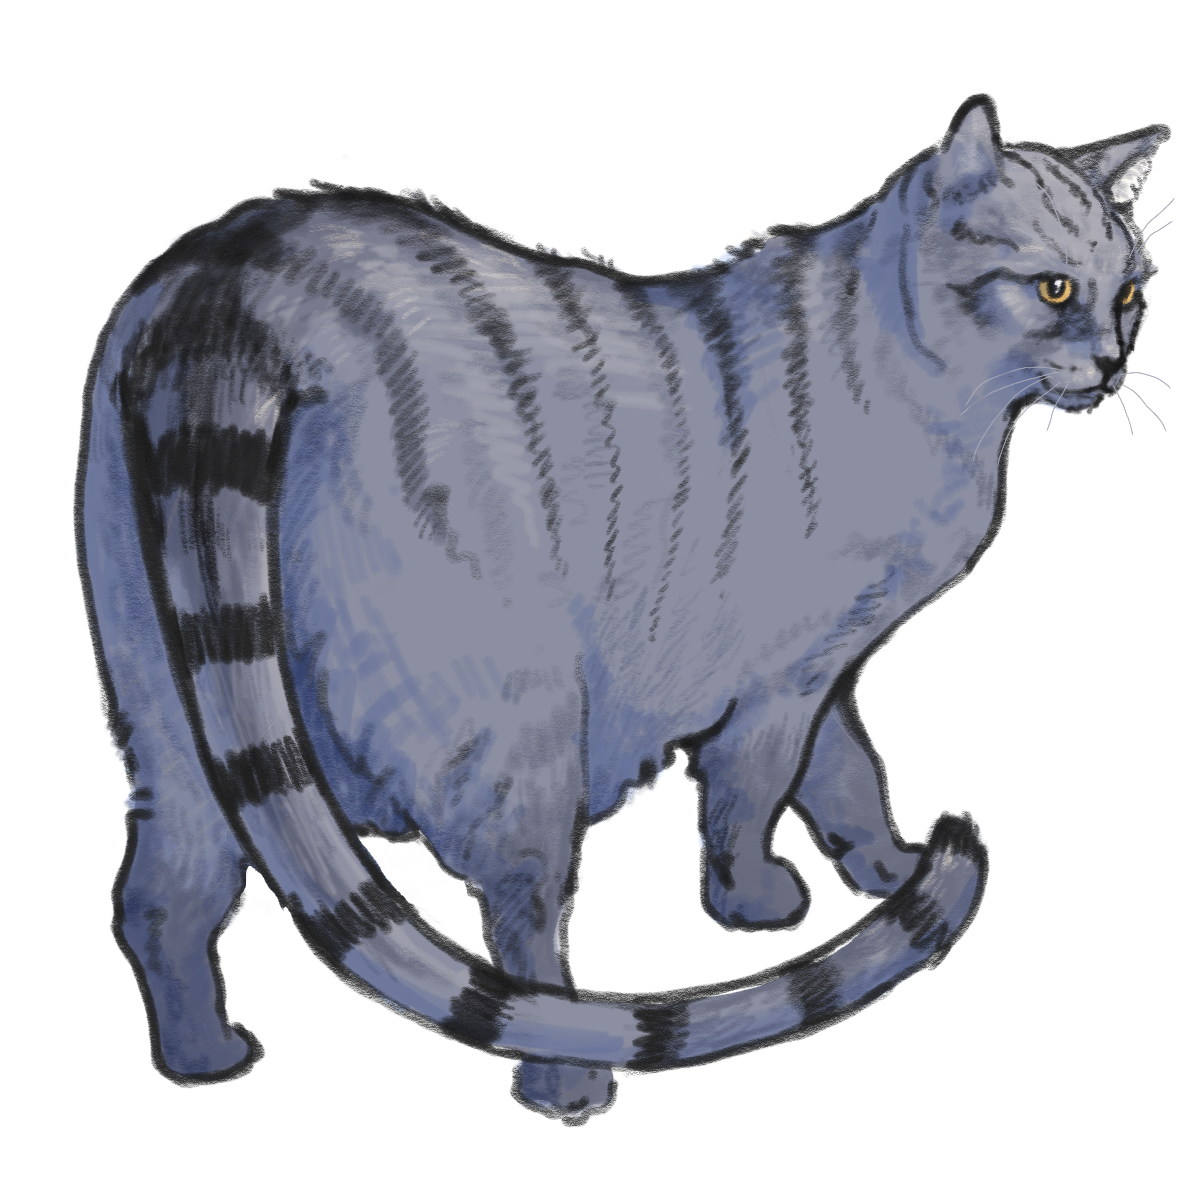
\includegraphics[width=2cm]{kot-bedlewo-full.png}};
    % \node[anchor=north] at (9.8, -9) {\scalebox{2}{\color{fg}\boldmath$\int$}};
    \node[anchor=north] at (12.2, -2) {\scalebox{-1}[1]{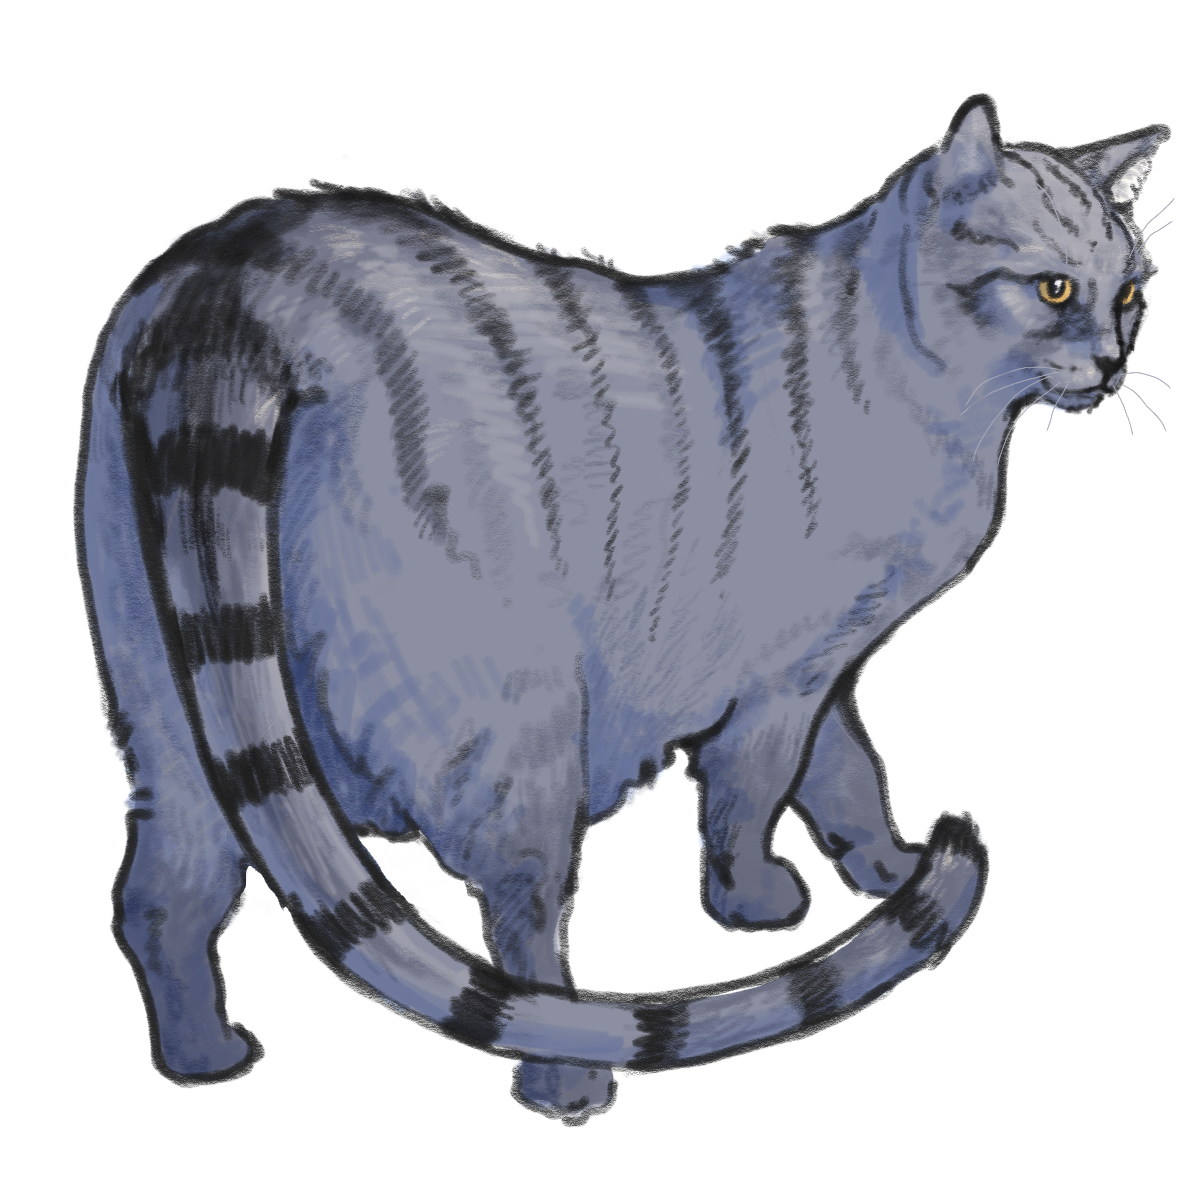
\includegraphics[width=3.3cm]{kot-bedlewo-full.png}}};
  \end{scope}

    \node[anchor=north west] (txt-1) at (.04\paperwidth, -4.7) {
        \begin{varwidth}{.91\paperwidth}\color{fg}\fontsize{15}{20}\selectfont
          The aim of the workshop is to prepare the next generation of mathematicians \linebreak to boldly go where no one has gone before by showing them research frontiers \linebreak in mathematics in a tangible and comprehensible way. It should reveal to students various possibilities for their research careers, both in terms of future research opportUniv.ies and the choice of potential thesis or postdoctoral advisors. \linebreak The workshop will combine \textbf{\color{yellow}15 expository lectures} by senior speakers, \textbf{\color{yellow}available online}, with presentations by participating students.
        \end{varwidth}
      };
  % speakers
  \begin{scope}[shift={(0, .2)}]

    \node[anchor=north west] (speakers) at (.04\paperwidth, -10.2) {
        \begin{varwidth}{.52\paperwidth}\color{fg}\fontsize{18}{25}\selectfont 
          \textbf{\color{orange}SPEAKERS:}
        \end{varwidth}
      };
    \node[anchor=north west] (speakers-list) at (.07\paperwidth, -11.2) {
        \begin{varwidth}{.53\paperwidth}\color{fg}
          \fontsize{14}{25}\selectfont \setlength{\parindent}{-1em} 
          \textbf{\color{yellow!50!fg}Francesco Bonsante} (Univ. of Pavia, Italy)
          
          \textbf{\color{yellow!50!fg}Jarosław Buczyński} (IMPAN, Warsaw, Poland)

          \textbf{\color{yellow!50!fg}Szymon Cygan} (Univ. of Wrocław, Poland)

          \textbf{\color{yellow!50!fg}Tomasz Downarowicz} (Wrocław Univ. of S\&T, Poland)

          \textbf{\color{yellow!50!fg}Urszula Foryś} (Univ. of Warsaw, Poland)

          \textbf{\color{yellow!50!fg}Piotr Kowalski} (Univ. of Wrocław, Poland)

          \textbf{\color{yellow!50!fg}Joanna Kułaga-Przymus} (NCU, Toruń, Poland)

          \textbf{\color{yellow!50!fg}Mateusz Kwaśnicki} (Wrocław Univ. of S\&T, Poland)

          \textbf{\color{yellow!50!fg}Laura Man\v cinska} (Univ. of Copenhagen, Denmark)

          \textbf{\color{yellow!50!fg}Krzysztof Meissner} (Univ. of Warsaw, Poland)

          \textbf{\color{yellow!50!fg}Piotr M. Sołtan} (Univ. of Warsaw, Poland)

          \textbf{\color{yellow!50!fg}Ravi Vakil} (Stanford Univ., USA)

          \textbf{\color{yellow!50!fg}Paul Wedrich} (Univ. of Hamburg, Germany)

          \textbf{\color{yellow!50!fg}Anna Wienhard} (MPI MIS, Leipzig, Germany)
          
          \textbf{\color{yellow!50!fg}Yizhe Zhu} (Univ. of California, Irvine, USA)
        \end{varwidth}
      };
  \end{scope}

  % organizers
  \begin{scope}[shift={(0,.2)}]
    \node[anchor=north] (organizers) at (.815\paperwidth ,-10.2) {\centering
        \color{orange}\bfseries\fontsize{18}{20}\selectfont
        ORGANIZERS:
      };
    \node[anchor=north] (organizers-list) at (.815\paperwidth, -11.2) {
        \begin{varwidth}{.3\paperwidth}\fontsize{14}{25}\selectfont\color{fg}\centering
          Ewa \textbf{\color{yellow!50!fg}Damek}
          
          Piotr M. \textbf{\color{yellow!50!fg}Hajac}

          Jacek \textbf{\color{yellow!50!fg}Miękisz}

          Adam \textbf{\color{yellow!50!fg}Wegert}
          
          Monika \textbf{\color{yellow!50!fg}Brattig}

          Weronika \textbf{\color{yellow!50!fg}Jakimowicz}
          
          Michał \textbf{\color{yellow!50!fg}Mądrala}

          Krzysztof \textbf{\color{yellow!50!fg}Szymański }

          Maciej \textbf{\color{yellow!50!fg}Frącek}

          Jakub \textbf{\color{yellow!50!fg}Krzysztoń}

          Maksymilian \textbf{\color{yellow!50!fg}Adamczewski}
        \end{varwidth}
      };
  \end{scope}
  
  \begin{scope}
    \foreach \i in {0,...,22} \fill[orange!50!fg, opacity=0.6] (.64\paperwidth, -10-.7*\i) circle (2 pt);
  \end{scope}

  \begin{scope}[shift={(.66\paperwidth,0)}]
    \node[anchor=west] (hybrydowe) at (0,-2) {\begin{varwidth}{0.29\paperwidth} \color{fg}\fontsize{23}{30}\selectfont\color{orange}
          Banach Center
          Będlewo, Poland
          \fontsize{19}{30}\selectfont
          \color{yellow}2-6 September 2024
        \end{varwidth}
      };
    % \node[anchor=west] at (0, -3) {\color{orange}available online};
  \end{scope}


  \begin{scope}[shift={(.34, -.2)}]
    \fill[lavender!10!fg, opacity=0.95] (-2, -0.88 * \paperheight) rectangle (\paperwidth+3, -\paperheight);
    % \fill[pattern={Dots[angle=30, radius=3pt, distance=15pt]}, pattern color=lavender!20!bg0, opacity=0.08] (-2,-.88*\paperheight) rectangle (\paperwidth+3, -\paperheight);
    \def\stopka{16mm}
    \def\posY{-.925\paperheight}

    \node[anchor=west] (banach) at (0.01\paperwidth, \posY) {
        
\includegraphics[height=\stopka]{bc_graphics.png}
      };
    
    \node[anchor=west] (impan) at (0.12\paperwidth, \posY) {
        \includesvg[height=\stopka]{impan-logo.svg} 
      };

    \node[anchor=west] at (0.51\paperwidth, \posY) (uwr) {
        \includesvg[height=\stopka]{uwr-logo.svg} 
      };
    \node[anchor=west] at (.78\paperwidth, \posY) {
        
\includegraphics[height=\stopka]{ptm-logo.png}
      };
  \end{scope}

%   \fill (.03\paperwidth, -.85\paperheight) circle (5pt);
% \fill (.25\paperwidth, -.9\paperheight) circle (5pt);
% \fill (10, -5) circle (5pt);


\end{tikzpicture}
\end{document}
